\begin{figure*}[!t]
    \subfloat[Average end-to-end performance]{
        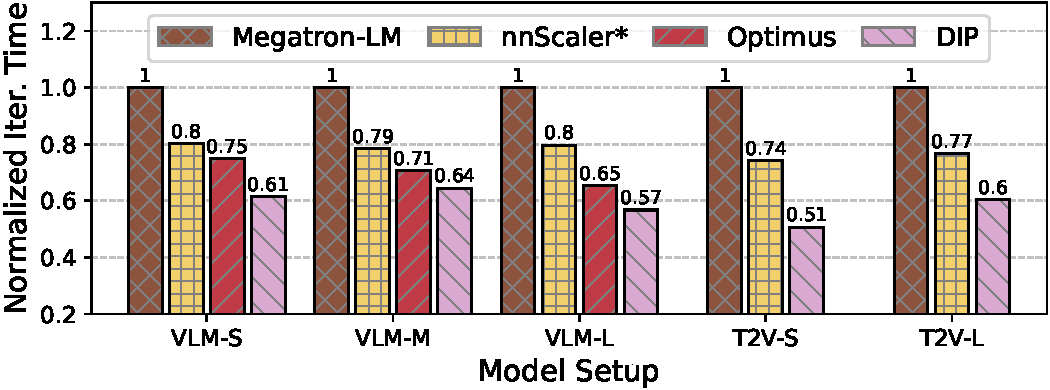
\includegraphics[height=29mm]{figures/weak_scaling.pdf}
    }
    \hfil
    \subfloat[Dynamic workloads]{
        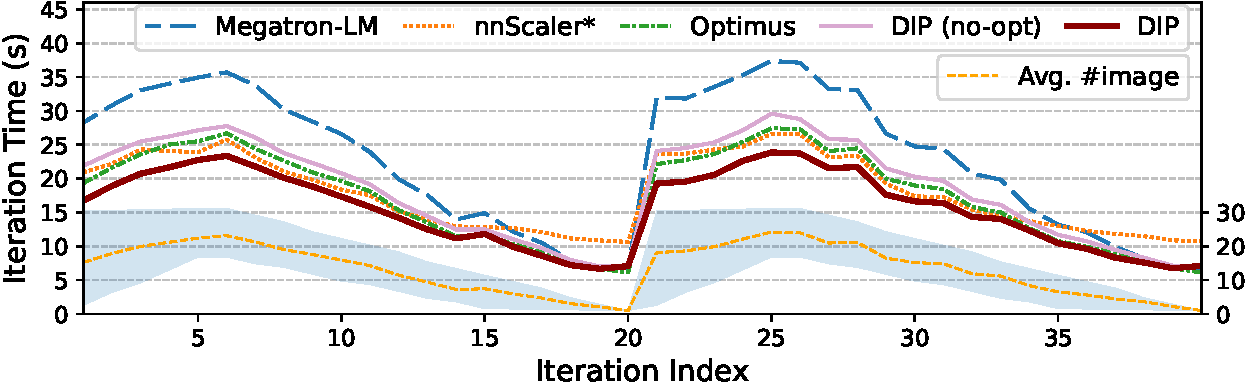
\includegraphics[height=29mm]{figures/dynamic_workload_timeline.pdf}
    }

    \caption{
        End-to-end performance.
        \textbf{(a)} Average performance of 100 iteration on real datasets across five model setups.
        \textbf{(b)} End-to-end latency timeline of 40 consecutive iterations.
        The orange dashed line depicts the average number of images.
    }
    \label{figure:e2e-perf}
\end{figure*}

\section{Evaluation}

\subsection{Methodology}
\label{section:datasets}

\heading{Models}
We conduct comprehensive evaluations of \sys{} across two major LMM architectures:
vision-language models (VLMs) and text-to-video (T2V) models (\tableref{table:model-params}).
The VLM architectures integrate ViT-based image encoders (5B and 22B parameters)~\cite{vit-iclr21,vit22b-arxiv23} with language model backbones (Llama3 8B~\cite{llama3-arxiv24}, Qwen2 32B/72B~\cite{qwen2-arxiv24}),
while T2V architectures combine language model encoders with DiT-based diffusion video decoders (5B and 30B parameters)~\cite{moviegen-arxiv24}.
We choose five distinct model combinations ranging from 12B to 94B parameters, as detailed in \tableref{table:model-setup}.

\heading{Datasets}
We employ a combination of diverse open-source datasets~\cite{obelics-arxiv23,laion5b-nips22,scienceqa-nips22,share-gpt4-video-arxiv24,internvid-arxiv23,mmtrail-arxiv24},
comprising pure image-text pairs, interleaved image-text documents, and video-caption pairs.
For VLM models, we adopt the ViT architecture used in Qwen2 VL~\cite{qwen2-vl-arxiv24}. We scale all images to 728px resolution, with each image being encoded by the ViT vision encoder into 169 patch tokens (\texttt{patch\_size}=14, \texttt{spatial\_merge\_size}=4).
Multiple image-text data samples are packed into sequences of 8192 tokens, resulting in a maximum image capacity of $\lfloor 8192/169 \rfloor=48$ per sequence.
For T2V models, we adopt MovieGen's~\cite{moviegen-arxiv24} configuration by transcoding videos to 16 FPS with a maximum duration of 16 seconds.
When processing short videos, we group up to 8 video clips per microbatch while maintaining the total microbatch duration below 16 seconds.

\heading{Baselines}
We benchmark \sys{} against four state-of-the-art baseline systems:

\begin{itemize}
    \item \textbf{Fully Sharded Data Parallel (FSDP)}~\cite{fsdp-arxiv23} is a memory-efficient training strategy standard in PyTorch. It shards model parameters, gradients, and optimizer states across data parallel workers, collecting them via communication only during the computation of the current layer.
    We employ FSDP2 in PyTorch 2.8.0 with ZeRO-3 configuration (\texttt{reshard\_after\_forward=true}) for Transformer blocks to minimize peak memory usage.
    \item \textbf{Megatron-LM}~\cite{megatron-lm-arxiv20} is a widely-used unimodal LLM training framework.
    We use interleaved pipeline parallelism (VPP) and partition LMM layers into model chunks with approximately balanced parameter distribution.
    \item \textbf{nnScaler}~\cite{nnscaler-osdi24}
    automates parallelization for deep neural network training.
    Since generating a single parallelization plan takes several minutes and requires a restart of the training process for plan updates,
    we pre-generate a static parallelization plan before training with a representative training workload.
    For fair cross-framework comparison, we implement nnScaler's model chunk partitioning schemes and memory optimizations in Megatron-LM,
    with performance metrics labeled as ``nnScaler*''.
    \item \textbf{Optimus}~\cite{optimus-atc25}
    proposes coarse-grained and fine-grained bubble scheduling
    to optimize multimodal LLM (MLLM) training with multiple encoders.
    The coarse-grained strategy sequences all modality encoder computations before backbone model execution at the pipeline level,
    while the fine-grained method fills TP communication bubbles with encoder computations
    and is orthogonal to our pipeline design.
    For focused pipeline scheduling comparisons, we implement Optimus' coarse-grained bubble scheduling in \sys{}.
    Due to the lack of support for diffusion decoders, we exclude Optimus from T2V model evaluations.
\end{itemize}

Spindle~\cite{spindle-asplos25} is excluded from the evaluation primarily because it is tailored for static, multi-task scenarios where tasks must be pre-defined prior to training.
This static design fundamentally contrasts with the dynamic and flexible input-handling capabilities required by modern LMMs.

\heading{Testbed}
We conducted large-scale experiments on a cluster of 64 NVIDIA 80GB H800 GPUs distributed across 8 nodes.
Each node is equipped with 128 CPU cores, 256GB of host memory,
and 8 H800 GPUs interconnected via 200 GB/s NVLink.
Inter-node communication relies on an 8$\times$200Gbps RoCEv2 network with a rail-optimized topology.
Additionally, a smaller cluster consisting of two nodes, each populated with 8 NVIDIA 96GB H20 GPUs,
was utilized for comparative baselines against FSDP and Megatron-LM.

\heading{Metrics}
We adopt training iteration time and model FLOPs utilization (MFU) as performance metrics, with all reported values averaged across 10 independent runs.

\subsection{End-to-End Performance}
\label{section:e2e-performance}

\heading{Comparison with LLM Training Systems}
We begin by benchmarking {\sys} against FSDP and Megatron-LM,
both of which are widely adopted frameworks for unimodal LLM training.
These experiments were conducted on the 16-GPU H20 cluster,
leveraging the large 96GB VRAM per GPU to minimize activation recomputation overhead.
As shown in \tableref{table:fsdp-comparison},
FSDP is only 3\% slower than Megatron-LM,
whereas {\sys} achieves a 27\% speedup over Megatron-LM.
Given the marginal performance gap between FSDP and Megatron-LM,
we implement all remaining baselines based on Megatron-LM to ensure a fair cross-framework comparison.

\begin{table}[t]
    \caption{
        VLM-S end-to-end performance of FSDP, Megatron-LM, and {\sys} on 16 H20 GPUs.
    }
    \label{table:fsdp-comparison}

    \small
    \begin{tabular}{>{\raggedright}lccc}
    \toprule
    & \textbf{FSDP}~\cite{fsdp-arxiv23} & \textbf{Megatron-LM}~\cite{megatron-lm-arxiv20} & \textbf{\sys} \\
    \midrule
    Iteration time (s) & 40.270 & 39.053 & 28.606 \\
    Relative time & 1.03 & 1.00 & 0.73 \\
    \bottomrule
    \end{tabular}
\end{table}

\heading{Comparison with Multimodal Training Systems}
We conduct experiments comparing the average end-to-end performance of \sys{} against baseline systems using real datasets and five model configurations summarized in \tableref{table:model-setup}.
As demonstrated in \figref{figure:e2e-perf}a, \sys{} achieves training throughput improvements of 15.6\%--76.2\% over three baseline systems in VLM model setups,
and 36.6\%--97.3\% over two baselines in T2V model configurations,
demonstrating consistent performance gains across diverse model architectures and parameter scales.

\heading{Dynamic Workloads}
To analyze \sys{}'s performance characteristics under dynamic workloads against other baselines,
we investigate the VLM-S model with manual control of image count bounds during training iterations.
We monitor 40 iterations showing two "rise-and-fall" patterns in image counts.
Each pattern consists of:
(1) gradually increasing the lower bound from 0 to 16 while maintaining an upper bound of 32 (iterations 1--5), achieving a peak average of 22 images,
followed by (2) progressively reducing both bounds to zero (iterations 6--20).

\figref{figure:e2e-perf}b reveals \sys{}'s consistent superior performance across all systems.
During high-image-count phases (iterations 1--10),
Megatron-LM suffers significant computational imbalance across modality modules and data microbatches,
exhibiting a 52.9\% slowdown compared to \sys{} at iteration 6.
Although both nnScaler and Optimus partially mitigate dynamic imbalance effects,
they are still 10.4\% slower than \sys{}.
As both image counts and bound gaps decrease (iterations 11--20),
training workloads converge toward pure language tasks,
narrowing the performance gap between \sys{} and baseline systems.
Notably, nnScaler's restriction to 1F1B scheduling mandates all modality modules to be partitioned inside one pipeline segment,
which creates significant pipeline imbalance when image encoder workloads diminish,
resulting in 50.5\% performance degradation during iterations 15--20.

\subsection{Performance Ablation}

\heading{Performance Breakdown}
Using the VLM-S model setup,
we incrementally integrate four key components
(modality-aware partitioner, pipeline stage interleaving, segment reordering, and per-layer memory optimization)
onto Megatron-LM.
As demonstrated in \tableref{table:performance-breakdown},
the modality-aware partitioner alone delivers a 17.3\% performance improvement over the baseline Megatron-LM,
highlighting its critical role in LMM training.
Among optimizations of pipeline schedule searcher,
pipeline stage interleaving provides a substantial 21.6\% performance boost compared to Megatron-LM's default pipelining.
Subsequent segment reordering and per-layer memory optimization enhance performance by an additional 23.9\%
via intelligent reordering of pipeline segments and adaptive memory optimization strategy selection.
In \figref{figure:e2e-perf}b, we visually contrast improvements from modality-aware partitioner and pipeline schedule searcher over dynamic workloads,
separated by the line labeled ``\sys{} (no-opt)'' that excludes pipeline schedule searcher's optimizations.

\begin{table}[t]
    \caption{
        Quantitative impact of \sys{}'s optimizations.
    }
    \label{table:performance-breakdown}

    \small
    \begin{tabular}{>{\raggedright}p{5cm}cc}
    \toprule
    \textbf{Techniques} & \textbf{Iter. Time (s)} & \textbf{$\Delta$\%} \\
    \midrule
    Vanilla Megatron-LM & 26.13 & 0.0\% \\
    \midrule
    + Modality-aware partitioner (\S\ref{section:modality-aware-partitioning}) & 22.27 & 17.3\% \\
    + Pipeline stage interleaving (\S\ref{section:stage-interleaving}) & 18.81 & 38.9\% \\
    + Pipeline segment reordering (\S\ref{section:segment-reordering}) & 17.61 & 48.3\% \\
    + Pre-layer memory optimization (\S\ref{section:memory-optimization}) & 16.05 & 62.8\% \\
    \bottomrule
    \end{tabular}
\end{table}

\heading{Impact of Sub-Microbatch Sizes}
We investigate the influence of modality-specific sub-microbatch sizes on pipeline scheduling and GPU execution efficiency using the VLM-S model,
by testing image sub-microbatch sizes ranging from 4 to 32 and deriving the best and the worst\footnote{We obtain the worst pipeline schedule by inverting the optimization goal of pipeline schedule searcher to maximizing iteration time.} pipeline schedules.

Our analysis of \figref{figure:pipeline-scheduling} reveals two key findings.
First, smaller sub-microbatch sizes (4--12) significantly reduce the performance gap between best and worst schedules from 15.4\% to 5.1\%.
This narrowed variance indicates reduced sensitivity to schedule configurations,
thereby lowering the difficulty in achieving optimal pipeline schedules.
Second, extremely small sub-microbatch sizes (<8) demonstrate diminishing returns due to underutilized GPU computational capacity,
resulting in a 12.1\% increase in iteration time compared to medium-sized batches.
Through empirical validation, we identify a sub-microbatch size of 12 as the optimal balance point between pipeline schedule flexibility and hardware utilization efficiency.

\begin{figure}[!t]
    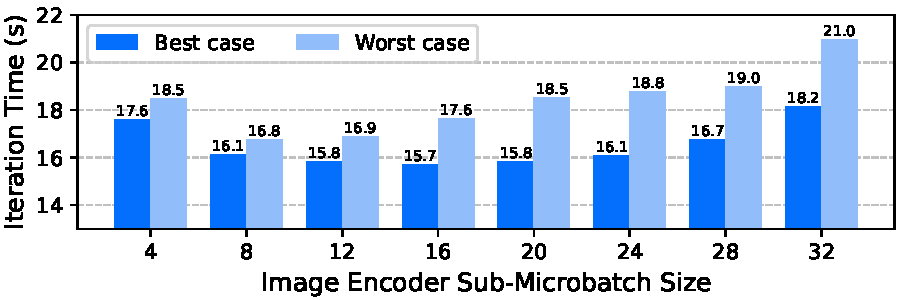
\includegraphics[width=1\columnwidth]{figures/pipeline_scheduling.pdf}
    \caption{
        Impact of sub-microbatch sizes.
    }
    \label{figure:pipeline-scheduling}
\end{figure}

\heading{Impact of Per-Layer Memory Optimization}
We analyze the memory usage timeline of the first pipeline rank during VLM-M model training.
As shown in \figref{figure:adaptive-computation},
baseline systems fail to fully utilize available GPU memory.
Megatron-LM exhibits significant memory fluctuations during the steady 1F1B pipeline phase,
while Optimus manifests a gradual memory increase due to executing all modality encoder computations and storing substantial activation memory prior to the backbone model.
This results in 25.3\% higher peak memory consumption compared to Megatron-LM.
In contrast, \sys{} maintains consistently low memory usage throughout training iterations
by partitioning microbatches into smaller sub-microbatches,
enabling finer-grained interleaving of forward and backward pipeline stages.
Per-layer memory optimization further intelligently selects memory optimization configurations
to achieve full utilization of available GPU memory,
achieving 52.9\% fewer memory fluctuations than Megatron-LM
and delivering 12.2\% performance gains over Optimus under equivalent peak memory conditions.

\begin{figure}[!t]
    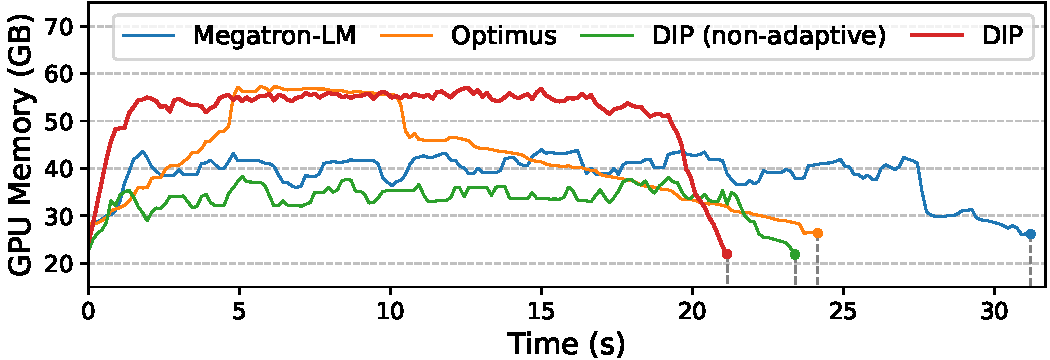
\includegraphics[width=1\columnwidth]{figures/adaptive_computation.pdf}
    \caption{
        Memory usage timelines of the first pipeline rank in VLM-M training.
        The ``\sys{} (non-adaptive)'' disables per-layer memory optimization and does not utilize all available GPU memory.
    }
    \label{figure:adaptive-computation}
\end{figure}

\begin{figure}[!t]
    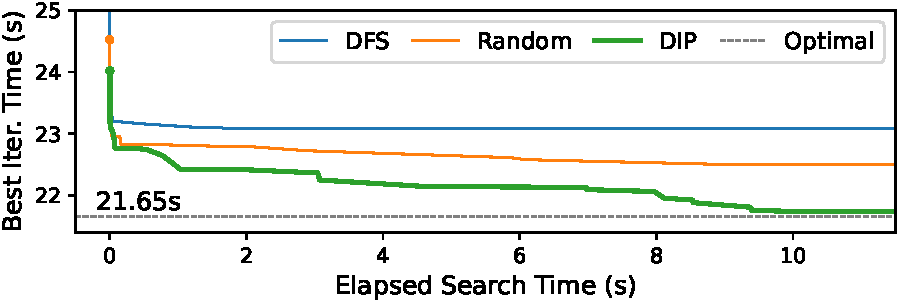
\includegraphics[width=1\columnwidth]{figures/search_efficiency.pdf}
    \caption{
        Search progress of different exploration strategies.
    }
    \label{figure:search-efficiency}
\end{figure}

\subsection{Planner Evaluation}
\label{section:planner-evaluation}

\heading{Search Efficiency}
To demonstrate the efficiency of \sys{}'s pipeline schedule search,
we track the progression of current best pipeline schedule performance versus elapsed search time,
comparing it with two variants using depth-first search (DFS) and random exploration
instead of MCTS algorithm.
Using the largest VLM-L model as the target workload, we run all search algorithm variants on 64 CPU cores.
\figref{figure:search-efficiency} shows \sys{} achieves near-optimal pipeline schedule performance within 10 seconds,
which can be overlapped with VLM-L's typical 20-second training iteration duration.
In contrast, DFS and random exploration strategies fail to quickly identify optimal pipeline schedules
due to their lack of guided search optimization with performance scores like MCTS.

\heading{Search Scalability}
We evaluate search scalability using two model configurations: VLM-S and T2V-S.
Specifically, we measure the search latency of {\sys} as the number of microbatches increases,
which correspondingly increases the number of pipeline stages and the complexity of the pipeline schedule.
We benchmark {\sys} against two state-of-the-art SMT/ILP solvers: Z3~\cite{z3} and Gurobi~\cite{gurobi} (version 13.0).
For the experimental setup, both {\sys} and Gurobi utilize up to 64 CPU threads,
whereas Z3 operates on a single thread as it inherently lacks support for multi-threaded solving.
As shown in \figref{figure:search-scalability}, {\sys} consistently maintains a search time under 10 seconds.
In contrast, the search times for both Z3 and Gurobi exhibit exponential growth with respect to the number of microbatches.
Consequently, both solvers cannot complete in 30 minutes when the number of microbatches surpasses 10,
rendering them impractical for dynamic pipeline schedule generation in LMM training.

\begin{figure}[!t]
    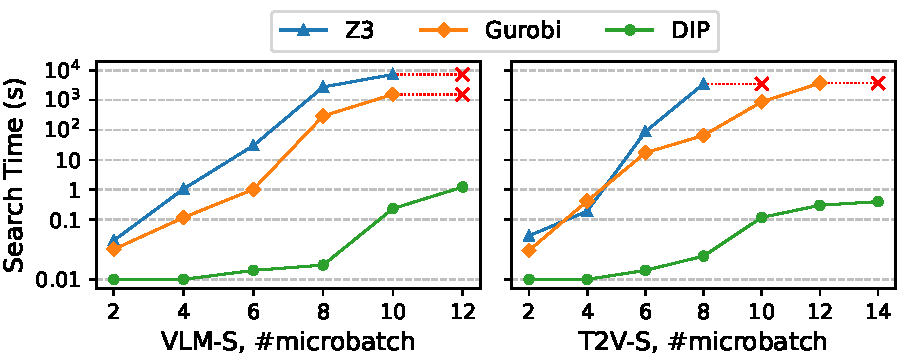
\includegraphics[width=1\columnwidth]{figures/search_scalability.pdf}
    \caption{
        Search time comparison of Z3, Gurobi, and {\sys} across varying microbatch counts for VLM-S and T2V-S.
        The Y-axis is plotted on a log scale.
        Red crosses (\textcolor{red}{$\times$}) indicate timeouts (>3 hours).
    }
    \label{figure:search-scalability}
\end{figure}

\heading{Simulation Accuracy}
We assess the accuracy of \sys{}'s training simulator through a grid-search experiment for VLM-M across 64 GPUs,
and compare simulated results against actual GPU executions.
We systematically evaluate all valid combinations of DP, PP, and TP sizes where all values are powers of two and TP $\leq 8$.
As illustrated in \figref{figure:simulation-accuracy},
the optimal parallelism configuration is DP8, TP2, and PP4, achieving a MFU of 29.7\%.
Although \sys{}'s default simulation settings initially exhibit relative errors up to 10\% compared to ground-truth measurements,
the simulator still successfully predicts the optimal parallel configuration.
Through calibration via offline microbenchmarks that align efficiency scaling factors for matrix multiplications and collective communication operations,
the training simulator achieves an average simulation accuracy of 97.6\%.

\begin{figure}[!t]
    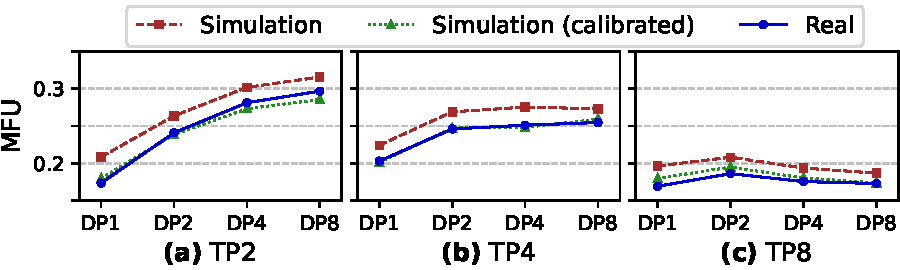
\includegraphics[width=1\columnwidth]{figures/simulation_accuracy.pdf}
    \caption{
        Comparison between pre- and post-calibration simulation results versus actual GPU executions.
    }
    \label{figure:simulation-accuracy}
\end{figure}

\subsection{Large-Scale Simulation}

To validate \sys{}'s effectiveness in large-scale H100 GPU cluster environments,
we conducted two experiments using the training simulator with substantial large multimodal models (VLM-XL and T2V-XL)
to evaluate its theoretical improvements over baseline approaches.
Detailed configurations for both models and GPU clusters are presented in \tableref{table:xl-model-setup}.

\begin{figure}[t]
    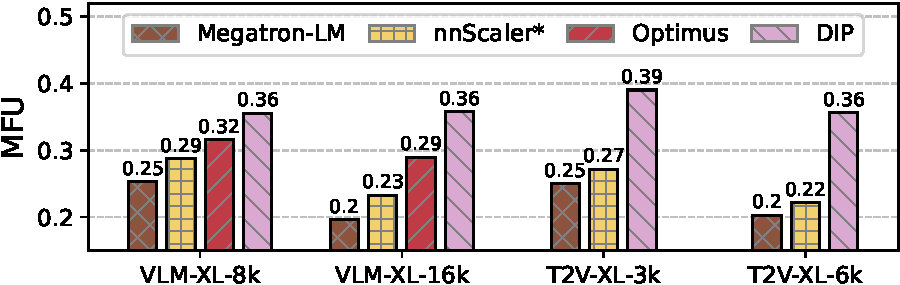
\includegraphics[width=1\columnwidth]{figures/large_scale_simulation.pdf}
    \caption{
        Large scale simulations on H100 clusters.
    }
    \label{figure:large-scale-simulation}
\end{figure}

\heading{Results}
Experimental results in \figref{figure:large-scale-simulation} demonstrate that \sys{} achieves MFU scores of 0.36 for VLM-XL and 0.39 for T2V-XL.
The system consistently outperforms baseline methods by up to 82.8\%,
particularly with larger pipeline parallelism sizes,
as larger PP dimensions introduce more complex pipeline structures
that require meticulous orchestration between stages by the pipeline schedule searcher.
